\begin{activity} \label{A:10.2.13} 
  Shown below in Figure \ref{F:10.2.activity.contour} is a contour
  plot of a function $f$.  The value of the function along a few
  of the contours is indicated to the left of the figure.

\begin{figure}[ht]
  \begin{center}
    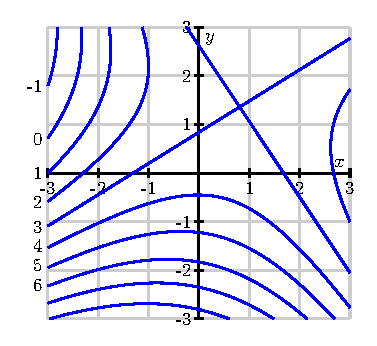
\includegraphics{figures/fig_10_2_activity_contours.eps}
    \caption{A contour plot of $f$.}
    \label{F:10.2.activity.contour}
  \end{center}
\end{figure}

\ba
\item Estimate the partial derivative $f_x(-2,-1)$.  
\item Estimate the partial derivative $f_y(-2,-1)$.
\item Estimate the partial derivatives $f_x(-1,2)$ and $f_y(-1,2)$.  
\item Locate one point $(x,y)$ where the partial derivative $f_x(x,y)=
  0$. 
\item Locate one point $(x,y)$ where $f_x(x,y)<0$.
\item Locate one point $(x,y)$ where $f_y(x,y)>0$.
\item Suppose you have a different function $g$, and you know that $g(2,2) =
  4$, $g_x(2,2) > 0$, and $g_y(2,2) > 0$.  Using this information,
  sketch a possibility for the contour $g(x,y)=4$ passing through
  $(2,2)$ on the left side of Figure \ref{F:10.2.activity.grad}.  Then
  include possible contours $g(x,y) = 3$ and $g(x,y) = 5$.

  \begin{figure}[ht]
    \begin{center}
      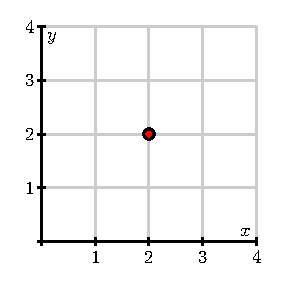
\includegraphics{figures/fig_10_2_activity_grad.eps}
      \hspace*{1in}
      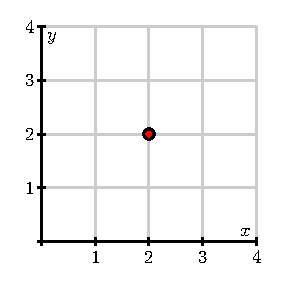
\includegraphics{figures/fig_10_2_activity_grad.eps}
    \end{center}
    \caption{Plots for contours of $g$ and $h$.}
    \label{F:10.2.activity.grad}
  \end{figure}
\item Suppose you have yet another function $h$, and you know that $h(2,2) =
  4$, $h_x(2,2) < 0$, and $h_y(2,2) > 0$.  Using this information,
  sketch a possible contour $h(x,y)=4$ passing through
  $(2,2)$ on the right side of Figure \ref{F:10.2.activity.grad}.
  Then include possible contours $h(x,y) = 3$ and $h(x,y) = 5$.
    
\ea

\end{activity}

\begin{activitySolution}
\ba
\item Recall that 
\[f_x(x,y) = \lim_{h \to 0} \frac{f(x+h,y) - f(x,y)}{h},\]
which gives us the slope of the tangent line to the trace in the $x$ direction. We can approximate this slope with the slope of a secant line, choosing points equally spaced on both sides of $(x,y)$. In other words,
\[f_x(x,y) \approx \frac{f(x+h,y) - f(x-h,y)}{2h},\]
for small values of $h$. This is the symmetric difference quotient from calculus 1. 
Using $h=1$ and approximating values from the contour plot gives us  
\[f_x(-2, -1) \approx \frac{f(-1,-1)-f(-3,-1)}{2} \approx \frac{4.5-2.9}{2} = 0.8.\] 
\item We approximate $f_y(-2,-1)$ in the same way, using $h=1$ again. So 
\[f_y(-2,-1) \approx \frac{f(-2,0)-f(-2,-2)}{2} \approx \frac{2.4-6}{2} = -1.8.\]
\item As above, 
\begin{align*}
f_x(-1,2) &\approx \frac{f(0,2)-f(-2,2)}{2} \approx \frac{3-0.8}{2} = 1.1 \\
f_y(-1,2) &\approx \frac{f(-1,3)-f(-1,1)}{2} \approx \frac{2.1-2.3}{2} = -0.1.
\end{align*}
\item A point at which $f_x(x,y) = 0$ will occur when we have a horizontal tangent line. Such a point occurs near $(0,-0.5)$. 
\item A point at which $f_y(x,y) = 0$ will occur when we have a vertical tangent line. Such a point occurs near $(-1,2)$. 
\item We want a point at which $f$ is decreasing in the $x$-direction. Such a point is $(2,-2)$.
\item We want a point at which $f$ is increasing in the $y$-direction. Such a point is $(-1.2,-1)$.
\item A possible plot is shown at left below.
\item A possible plot is shown at right below.
    \begin{center}
      \resizebox{!}{2.0in}{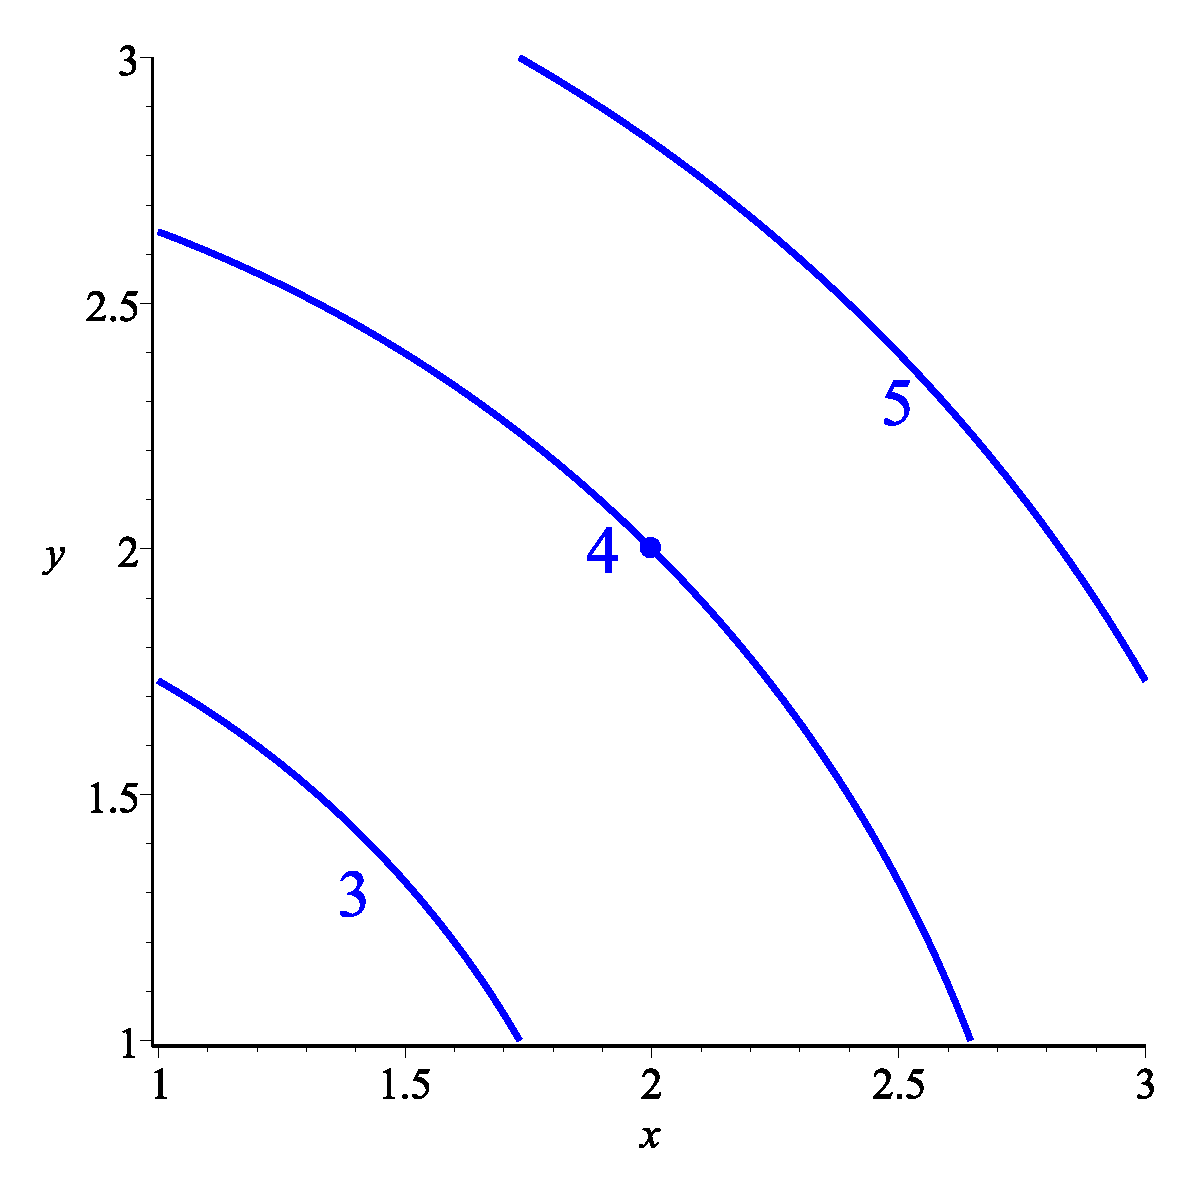
\includegraphics{figures/fig_10_2_activity_grad_g.eps}}
      \hspace*{1in}
      \resizebox{!}{2.0in}{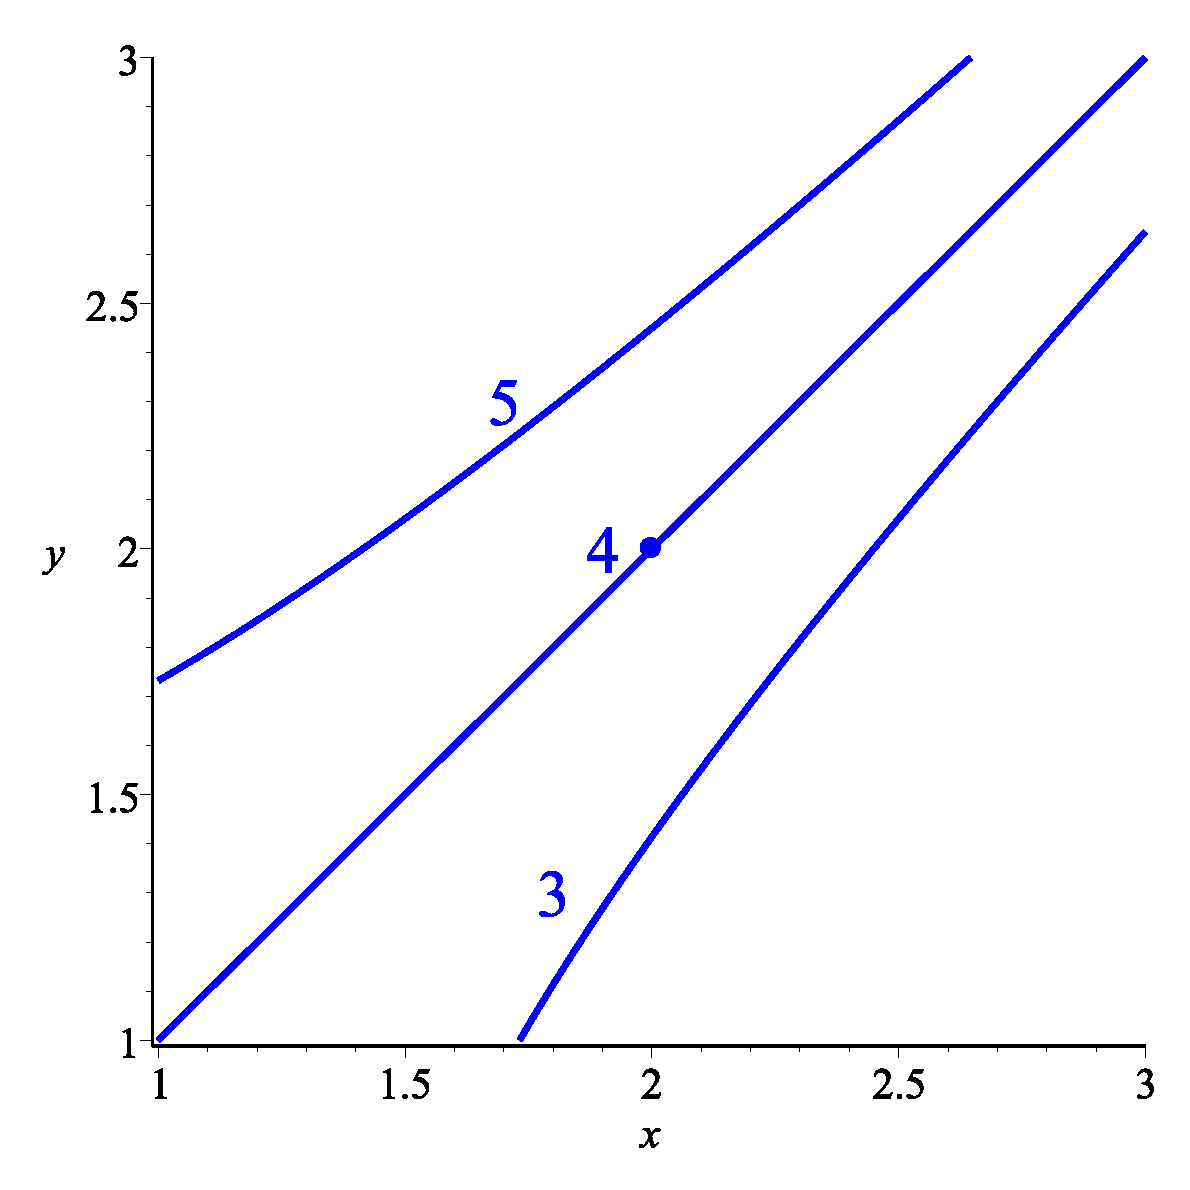
\includegraphics{figures/fig_10_2_activity_grad_h.eps}}
    \end{center}
\ea
\end{activitySolution}


\aftera
